\documentclass[xetex,mathserif,serif]{beamer}
\usepackage{polyglossia}
\setdefaultlanguage[babelshorthands=true]{russian}
\usepackage{minted}
\usepackage{tabu}

\useoutertheme{infolines}

\usepackage{fontspec}
\setmainfont{FreeSans}
\newfontfamily{\russianfonttt}{FreeSans}

\usepackage{textpos}
\setlength{\TPHorizModule}{1cm}
\setlength{\TPVertModule}{1cm}

\setbeamertemplate{blocks}[rounded][shadow=false]

\setbeamercolor*{block title alerted}{fg=red!50!black,bg=red!20}
\setbeamercolor*{block body alerted}{fg=black,bg=red!10}

\tabulinesep=1.2mm

\title[UML и анализ]{Лекция 4: UML и анализ}
\author[Юрий Литвинов]{Юрий Литвинов\\\small{\textcolor{gray}{yurii.litvinov@gmail.com}}}
\date{12.10.2017г}

\newcommand{\todo}[1] {
	\begin{center}\textcolor{red}{TODO: #1}\end{center}
}

\newcommand{\DownArrow} {
	\hspace{2cm}\begin{LARGE}$\downarrow$\end{LARGE}
}

\newcommand{\attribution}[1] {
	\vspace{-5mm}\begin{flushright}\begin{scriptsize}\textcolor{gray}{\textcopyright\, #1}\end{scriptsize}\end{flushright}
}

\begin{document}

	\frame{\titlepage}

	\section{Моделирование требований}

	\begin{frame}
		\frametitle{Моделирование требований}
		Первый этап разработки любой системы --- сбор и анализ требований
		\begin{itemize}
			\item Понимание разработчиками решаемой задачи
			\item Соглашение между разработчиками, заказчиками и пользователями
			\begin{itemize}
				\item Заказчики и пользователи часто разные люди с разными потребностями
			\end{itemize}
			\item Чёткое обозначение границ системы
			\item Основа для планирования проекта
			\item Чаще всего словесное описание требований, реже формальные модели
		\end{itemize}
	\end{frame}

	\begin{frame}
		\frametitle{Диаграмма случаев использования UML}
		\framesubtitle{Диаграмма прецедентов}
		\begin{columns}
			\begin{column}{0.5\textwidth}
				\begin{itemize}
					\item Ивар Якобсон, 1992 год
					\item Акторы (или актёры, роли) --- внешние сущности, использующие систему
					\begin{itemize}
						\item Люди или другие программные системы
					\end{itemize}
					\item Случаи использования (прецеденты)  --- цель использования системы актором
					\begin{itemize}
						\item Раскрываются в набор сценариев, описываемых чаще текстом
					\end{itemize}
				\end{itemize}
			\end{column}
			\begin{column}{0.5\textwidth}
				\begin{center}
					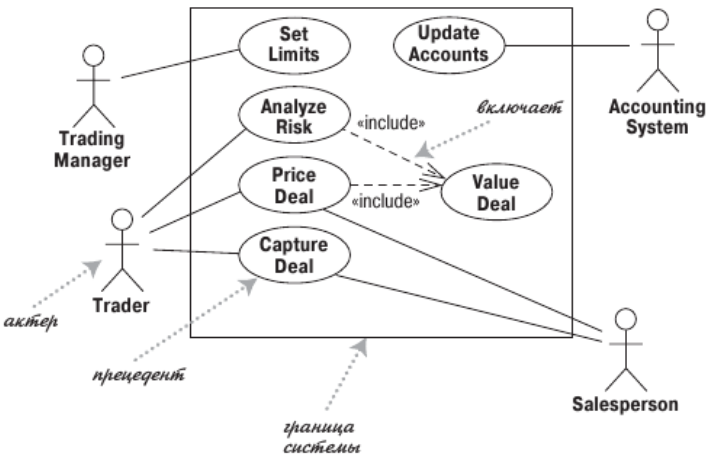
\includegraphics[width=\textwidth]{useCaseDiagram.png}
					\attribution{М. Фаулер, UML. Основы}
				\end{center}
			\end{column}
		\end{columns}
	\end{frame}

	\begin{frame}
		\frametitle{Include и Extend}
		Include:
		\begin{center}
			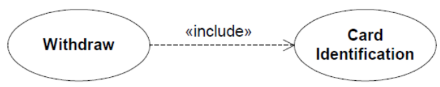
\includegraphics[width=0.45\textwidth]{useCaseInclude.png}
		\end{center}
		\vspace{5mm}
		Extend:
		\begin{center}
			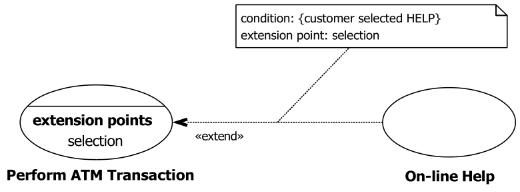
\includegraphics[width=0.5\textwidth]{useCaseExtend.png}
		\end{center}
		\attribution{OMG, UML 2.5 Specification}
	\end{frame}

	\begin{frame}
		\frametitle{Пример, check-in в аэропорту}
		\begin{center}
			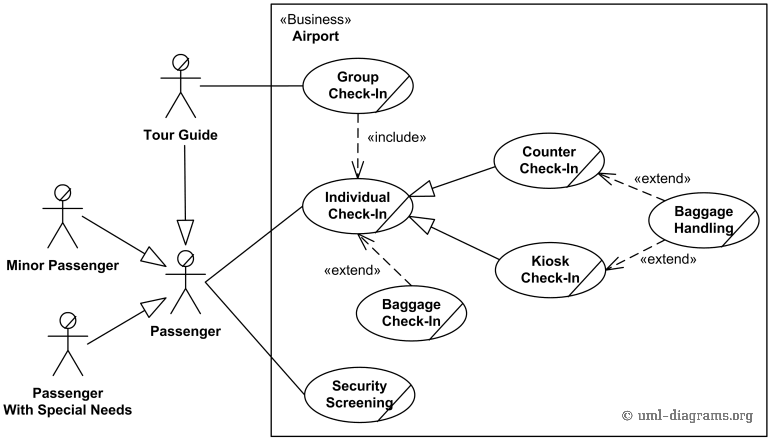
\includegraphics[width=0.7\textwidth]{airportUseCase.png}
			\attribution{http://www.uml-diagrams.org}
		\end{center}
	\end{frame}

	\begin{frame}
		\frametitle{Случай использования, типичная структура}
		\begin{itemize}
			\item Заголовок (цель основного актора)
			\item Заинтересованые лица, акторы, основной актор
			\item Предусловия
			\item Триггеры (активаторы)
			\item Основной порядок событий
			\item Альтернативные пути и расширения
			\item Постусловия
		\end{itemize}
	\end{frame}

	\begin{frame}
		\begin{center}
			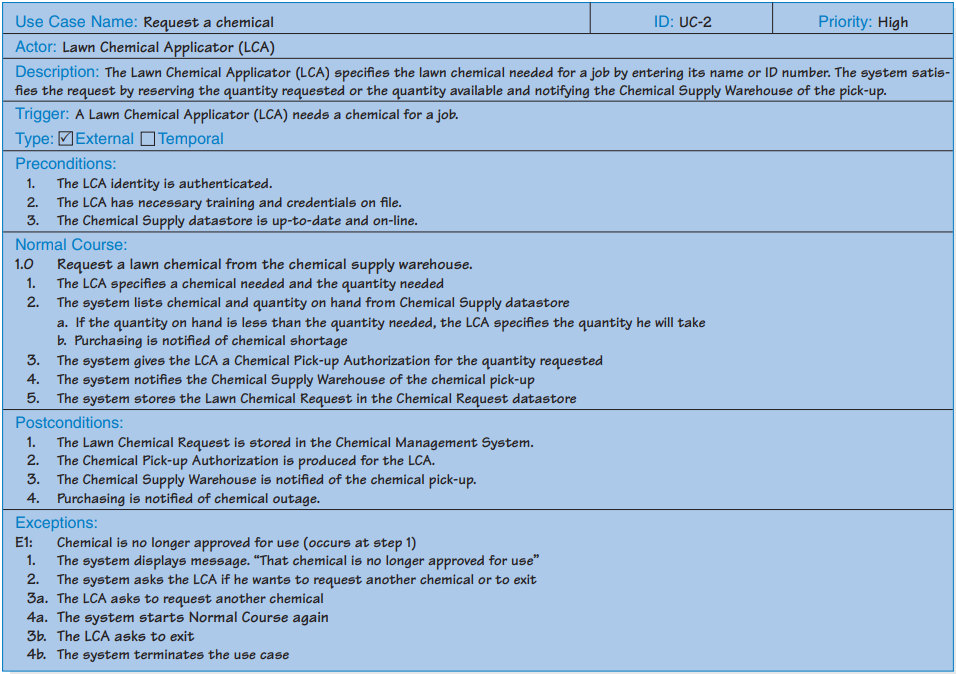
\includegraphics[width=0.9\textwidth]{useCaseExample.png}
			\attribution{R.M. Roth et al., System Analysis and Design}
		\end{center}
	\end{frame}

	\section{CASE-системы}
	
	\begin{frame}
		\frametitle{Computer-Aided Software Engineering}
		\begin{itemize}
			\item В 80-е годы термином CASE называли всё, что помогает разрабатывать ПО с помощью компьютера
			\begin{itemize}
				\item Даже текстовые редакторы
			\end{itemize}
			\item Теперь --- прежде всего средства для визуального моделирования (UML-диаграммы, ER-диаграммы и т.д.)
			\item Отличаются от графических редакторов тем, что ``понимают'', что в них рисуют
			\item Нынче чаще используются термины ``MDE tool'', ``UML tool'' и т.д.
		\end{itemize}
	\end{frame}

	\begin{frame}
		\frametitle{Типичная функциональность CASE-инструментов}
		\begin{itemize}
			\item Набор визуальных редакторов
			\item Репозиторий
			\item Набор генераторов
			\item Текстовый редактор
			\item Редактор форм
			\item Средства обратного проектирования (reverse engineering)
			\item Средства верификации и анализа моделей
			\item Средства эмуляции и отладки
			\item Средства обеспечения командной разработки
			\item API для интеграции с другими инструментами
			\item Библиотеки шаблонов и примеров
		\end{itemize}
	\end{frame}

	\begin{frame}
		\frametitle{Примеры CASE-инструментов}
		\begin{itemize}
			\item ``Рисовалки''
			\begin{itemize}
				\item Visio
				\item Dia
				\item SmartDraw
				\item Creately
			\end{itemize}
			\item Полноценные CASE-системы
			\begin{itemize}
				\item Enterprise Architect
				\item Rational Software Architect
				\item MagicDraw
				\item Visual Paradigm
				\item GenMyModel
			\end{itemize}
			\item Забавные штуки
			\begin{itemize}
				\item \url{https://www.websequencediagrams.com/}
				\item \url{http://yuml.me/}
				\item \url{http://plantuml.com/}
			\end{itemize}
		\end{itemize}
	\end{frame}

\end{document}
